\documentclass[tikz,border=5pt]{standalone}
\usepackage{tikz}
\usepackage{amsmath}
\usetikzlibrary{arrows.meta}
\definecolor{nebula}{HTML}{6366F1}
\definecolor{spark}{HTML}{14B8A6}
\definecolor{ink}{HTML}{334155}
\begin{document}
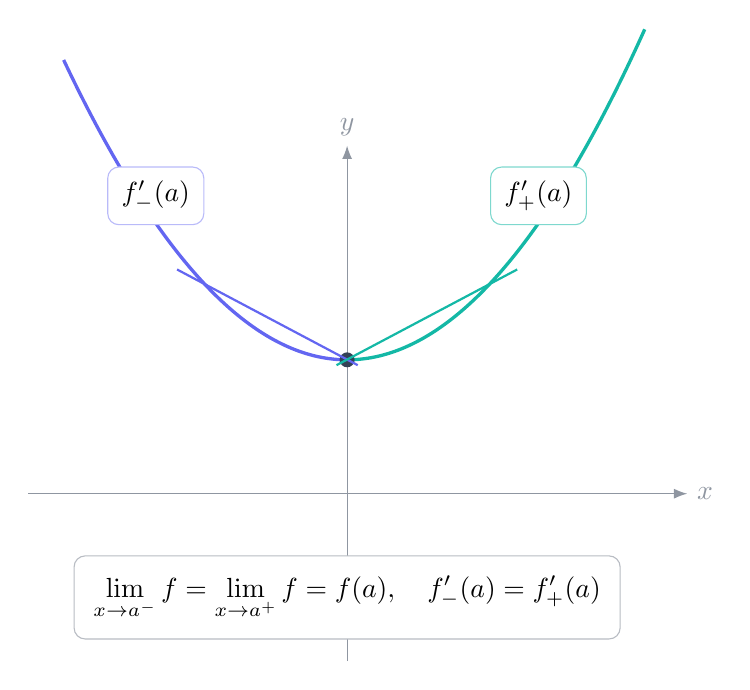
\begin{tikzpicture}[font=\sffamily,>=Latex,x=.9cm,y=.85cm]
  \draw[->,ink!55] (-4.5,0)--(4.8,0) node[right] {$x$};
  \draw[->,ink!55] (0,-2.5)--(0,5.2) node[above] {$y$};
  \draw[very thick,nebula,domain=-4:0,samples=100,smooth] plot(\x,{.28*\x*\x+2});
  \draw[very thick,spark,domain=0:4.2,samples=100,smooth] plot(\x,{.28*\x*\x+2});
  \fill[ink] (0,2) circle (2.7pt);
  \draw[nebula,thick] (-2.4,3.35)--(.15,1.92);
  \draw[spark,thick] (-.15,1.92)--(2.4,3.35);
  \node[draw=nebula!45,rounded corners=4pt,fill=white,inner sep=5pt] at (-2.7,4.45) {$f'_-(a)$};
  \node[draw=spark!55,rounded corners=4pt,fill=white,inner sep=5pt] at (2.7,4.45) {$f'_+(a)$};
  \node[draw=ink!35,rounded corners=4pt,fill=white,inner sep=7pt] at (0,-1.55)
    {$\displaystyle \lim_{x\to a^-}f=\lim_{x\to a^+}f=f(a),\quad f'_-(a)=f'_+(a)$};
\end{tikzpicture}
\end{document}
